%!TEX root = main.tex

\section{Prioritized Streaming String Transducers}  \label{sect:psst}
%\zhilin{Move from preliminary to here}

In this section, we introduce prioritized streaming string transducers (PSST), which extends prioritized finite-state automata (PFA) proposed in \cite{BM17}. We shall utilize PSST to model  the eager and greedy semantics of $\regexp$ as well as the behavior of $\replaceall$ functions where both capturing groups and back references occur.
%based on which we model the semantics of $\regexp$ defined in Section~\ref{sec:prel} and design the decision procedure in Section~\ref{sec:decision}.

%\paragraph{Prioritized Finite-state automata.}
%
For a finite set $Q$, let $\overline{Q} = \bigcup_{n\in \Nat}\{ (q_1, \ldots, q_n) \mid \forall i \in [n], q_i \in Q \wedge \forall i,j \in[n], i \neq j \rightarrow q_i \neq q_j \}$. Intuitively, $\overline{Q}$ is the set of sequences of non-repetitive elements from $Q$. In particular, the empty sequence $\varepsilon \in \overline{Q}$. Note that the length of each sequence from $\overline{Q}$ is bounded by  $| Q |$. For a sequence $P = (q_1, \ldots, q_n) \in \overline{Q}$ and  $q \in Q$, we write $q \in P$ if  $q = q_i$ for some $i \in [n]$. Moreover, for $P_1 = (q_1, \ldots, q_m) \in \overline{Q}$ and $P_2 = (q'_1, \ldots, q'_n) \in \overline{Q}$, we say $P_1 \cap P_2 = \emptyset$ if $\{q_1, \ldots, q_m\} \cap \{q'_1, \ldots, q'_n\} = \emptyset$.


\begin{definition}[Prioritized Finite-state Automata]\label{def-pfa}
  A \emph{prioritized finite-state automaton} (PFA) over a finite alphabet $\Sigma$ is a tuple $\pnfa=(Q, \Sigma, \delta, \tau, q_0, F)$ where $\delta \in Q
  \times \Sigma \rightarrow \overline{Q}$ and $\tau \in Q \rightarrow \overline{Q} \times \overline{Q}$ such that for every $q \in Q$, if $\tau(q) = (P_1; P_2)$, then $P_1 \cap P_2 = \emptyset$. 
  The definition of $Q$, $q_0$ and $F$ is the same as ordinary FA.
\end{definition}
For $\tau(q) = (P_1; P_2)$, we will use $\pi_1(\tau(q))$ and $\pi_2(\tau(q))$ to denote $P_1$ and $P_2$ respectively.  With slight abuse of notation, we write $q\in (P_1; P_2)$ for $q\in P_1\cup P_2$. Intuitively, $\tau(q)=(P_1; P_2)$ specifies the $\varepsilon$-transitions at $q$, with the intention that the $\varepsilon$-transitions to the states in $P_1$ resp. $P_2$ have higher resp. lower priorities than the non-$\varepsilon$-transitions out of $q$.
  
A  run of $\pnfa$ on a string $w$ is a sequence $q_0 \sigma'_1 q_1 \ldots \sigma'_m q_m$ such that 
\begin{itemize}
%\item $q_m \in F$,
\item for any $i \in [m]$, either $\sigma'_i \in \Sigma$ and $q_i \in \delta (q_{i - 1}, \sigma'_i)$, or $\sigma'_i = \varepsilon$ and $q_i \in \tau(q_{i-1})$ %\pi_1(\tau(q_{i-1}))\cup \pi_2(\tau(q_{i-1}))$,
\item $w = \sigma'_1 \cdots \sigma'_m$,
%
\item for every subsequence $q_i \sigma'_{i+1} q_{i+1} \ldots \sigma'_{j} q_j$ such that  $i < j$ and $\sigma'_{i+1} = \cdots = \sigma'_j = \varepsilon$, it holds that for every $k, l: i \le k < l < j$, $(q_k, q_{k+1}) \neq (q_l, q_{l+1})$.
%each state $q \in Q$ occurs \emph{at most twice} in the subsequence. 
(Intuitively, each transition occurs at most once in a sequence of $\varepsilon$-transitions.) 
\end{itemize}
Note that it is possible that $\delta(q, \sigma) = ()$, namely, there is no $\sigma$-transition out of $q$. 
It is easy to observe that given a string $w$, the length of a run of $\pnfa$ on $w$ is $O(|w||\cA|)$.
For any two runs $p = q_0 \sigma_1 q_1 \ldots \sigma_m q_m$ and $p' =  q_0 \sigma'_1 q_1' \ldots \sigma'_n q'_n$ such that $\sigma_1 \ldots \sigma_m = \sigma'_1 \ldots \sigma'_n$, we say that $p$ is of a higher priority over $p'$ if 
\begin{itemize}
\item either $p'$ is a prefix of $p$ (in this case, the transitions of $p$ after $p'$ are all $\varepsilon$-transitions), 
%
\item or there is an index $j$ satisfying one of the following constraints:
\begin{itemize}
\item $q_0 \sigma_1 q_1 \ldots q_{j-1} \sigma_j = q_0 \sigma'_1 q'_1 \ldots q'_{j-1} \sigma'_j$, $q_j \neq q'_j$, $\sigma_j \in \Sigma$, and $\delta (q_{j - 1}, \sigma_j) =(\ldots, q_j, \ldots, q_j', \ldots)$,
%
\item $q_0 \sigma_1 q_1 \ldots q_{j-1} \sigma_j = q_0 \sigma'_1 q'_1 \ldots q'_{j-1} \sigma'_j$, $q_j \neq q'_j$, $\sigma_j  = \varepsilon$,  and  either $\pi_1(\tau(q_{j - 1})) = (\ldots, q_j, \ldots, q_j', \ldots)$, or $\pi_2(\tau(q_{j - 1})) = (\ldots, q_j, \ldots, q_j', \ldots)$, or $q_j \in \pi_1(\tau(q_{j - 1}))$ and $q'_j \in \pi_2(\tau(q_{j-1}))$, 
%
\item $q_0 \sigma_1 q_1 \ldots q_{j-1}  = q_0 \sigma'_1 q'_1 \ldots q'_{j-1} $, $\sigma_j  = \varepsilon$, $\sigma'_j  \in \Sigma$, $q_j \in \pi_1(\tau(q_{j - 1}))$, and $q'_j \in \delta(q_{j-1}, \sigma'_j)$, 
%
\item $q_0 \sigma_1 q_1 \ldots q_{j-1}  = q_0 \sigma'_1 q'_1 \ldots q'_{j-1} $, $\sigma_j  \in \Sigma$, $\sigma'_j  = \varepsilon$, $q_j \in \delta(q_{j - 1}, \sigma_j)$, and $q'_j \in \pi_2(\tau(q_{j-1}))$.
\end{itemize}
\end{itemize}

An \emph{accepting} run of $\pnfa$ on $w$ is a run $q_0 \sigma_1 q_1 \ldots \sigma_m q_m$ of $\pnfa$ on $w$ with the \emph{highest} priority such that $q_m \in F$. (Note that a run $q_0 \sigma_1 q_1 \ldots \sigma_m q_m$ of $\pnfa$ with the highest priority may not be accepting, i.e. satisfy $q_m \in F$.) The language of $\pnfa$, denoted as $\Lang(\pnfa)$, is the set of strings on which $\pnfa$ has an accepting run.


Note that PFAs differ from FAs only in the way that the strings are accepted, they still define regular languages. 

%\begin{figure}[ht]
%\centering
%\rule{\linewidth}{0cm}
%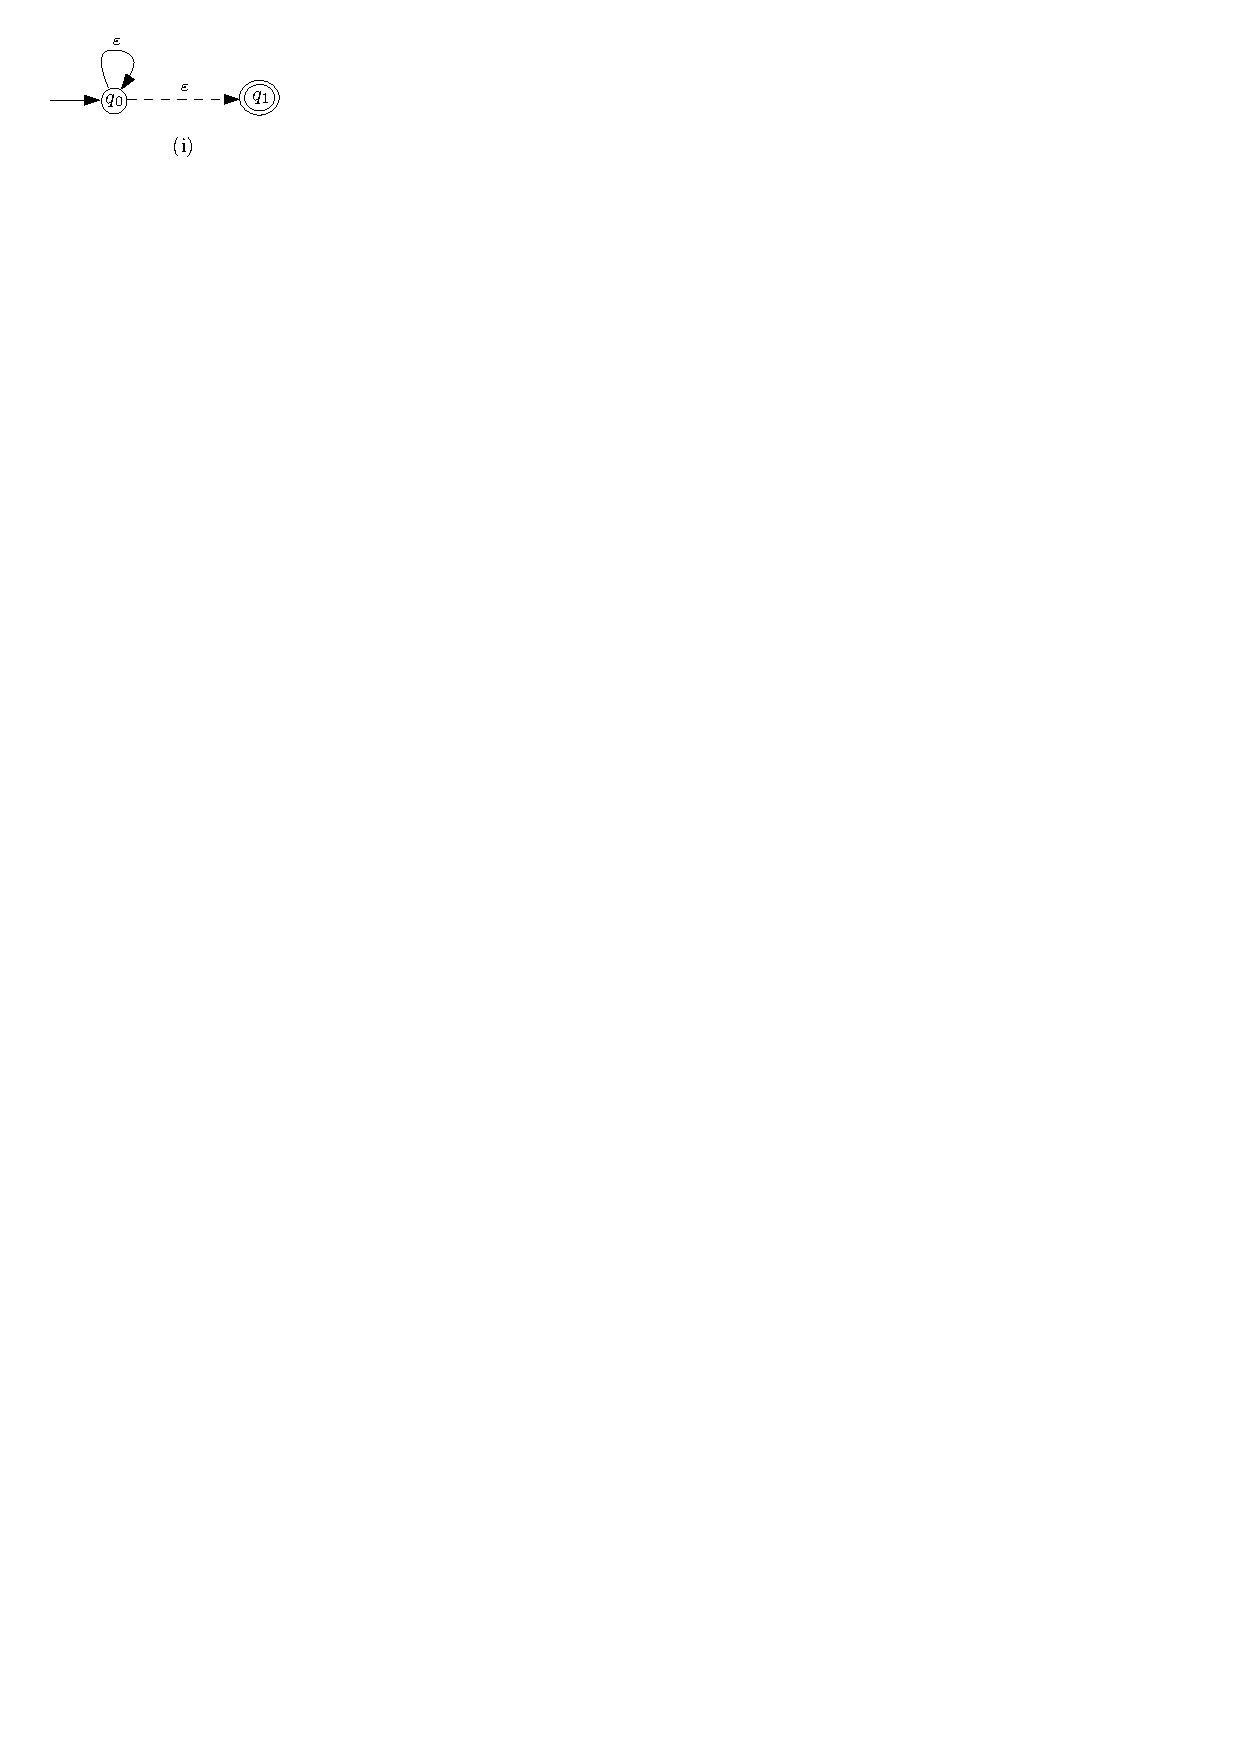
\includegraphics[scale=0.8]{pfa-epsilon-star.pdf}
%\caption{The PFA for $\varepsilon^\ast$}
%\label{fig-pfa-epsilon-star}
%\end{figure}

\begin{example}\label{exmp-pfa}
The PFAs corresponding to $a^\ast$ and $a^{\ast?}$ respectively are illustrated in Figure~\ref{fig-pfa}: (i) and (ii), where the dashed line represents $\pi_2(\tau(q_0))$ (of lower priority than the $a$-transition), the thicker solid line represents $\pi_1(\tau(q_0))$ (of higher priority than the $a$-transition), and the doubly circled state $q_1$ is a final state.

\begin{figure}[ht]
\centering
%\rule{\linewidth}{0cm}
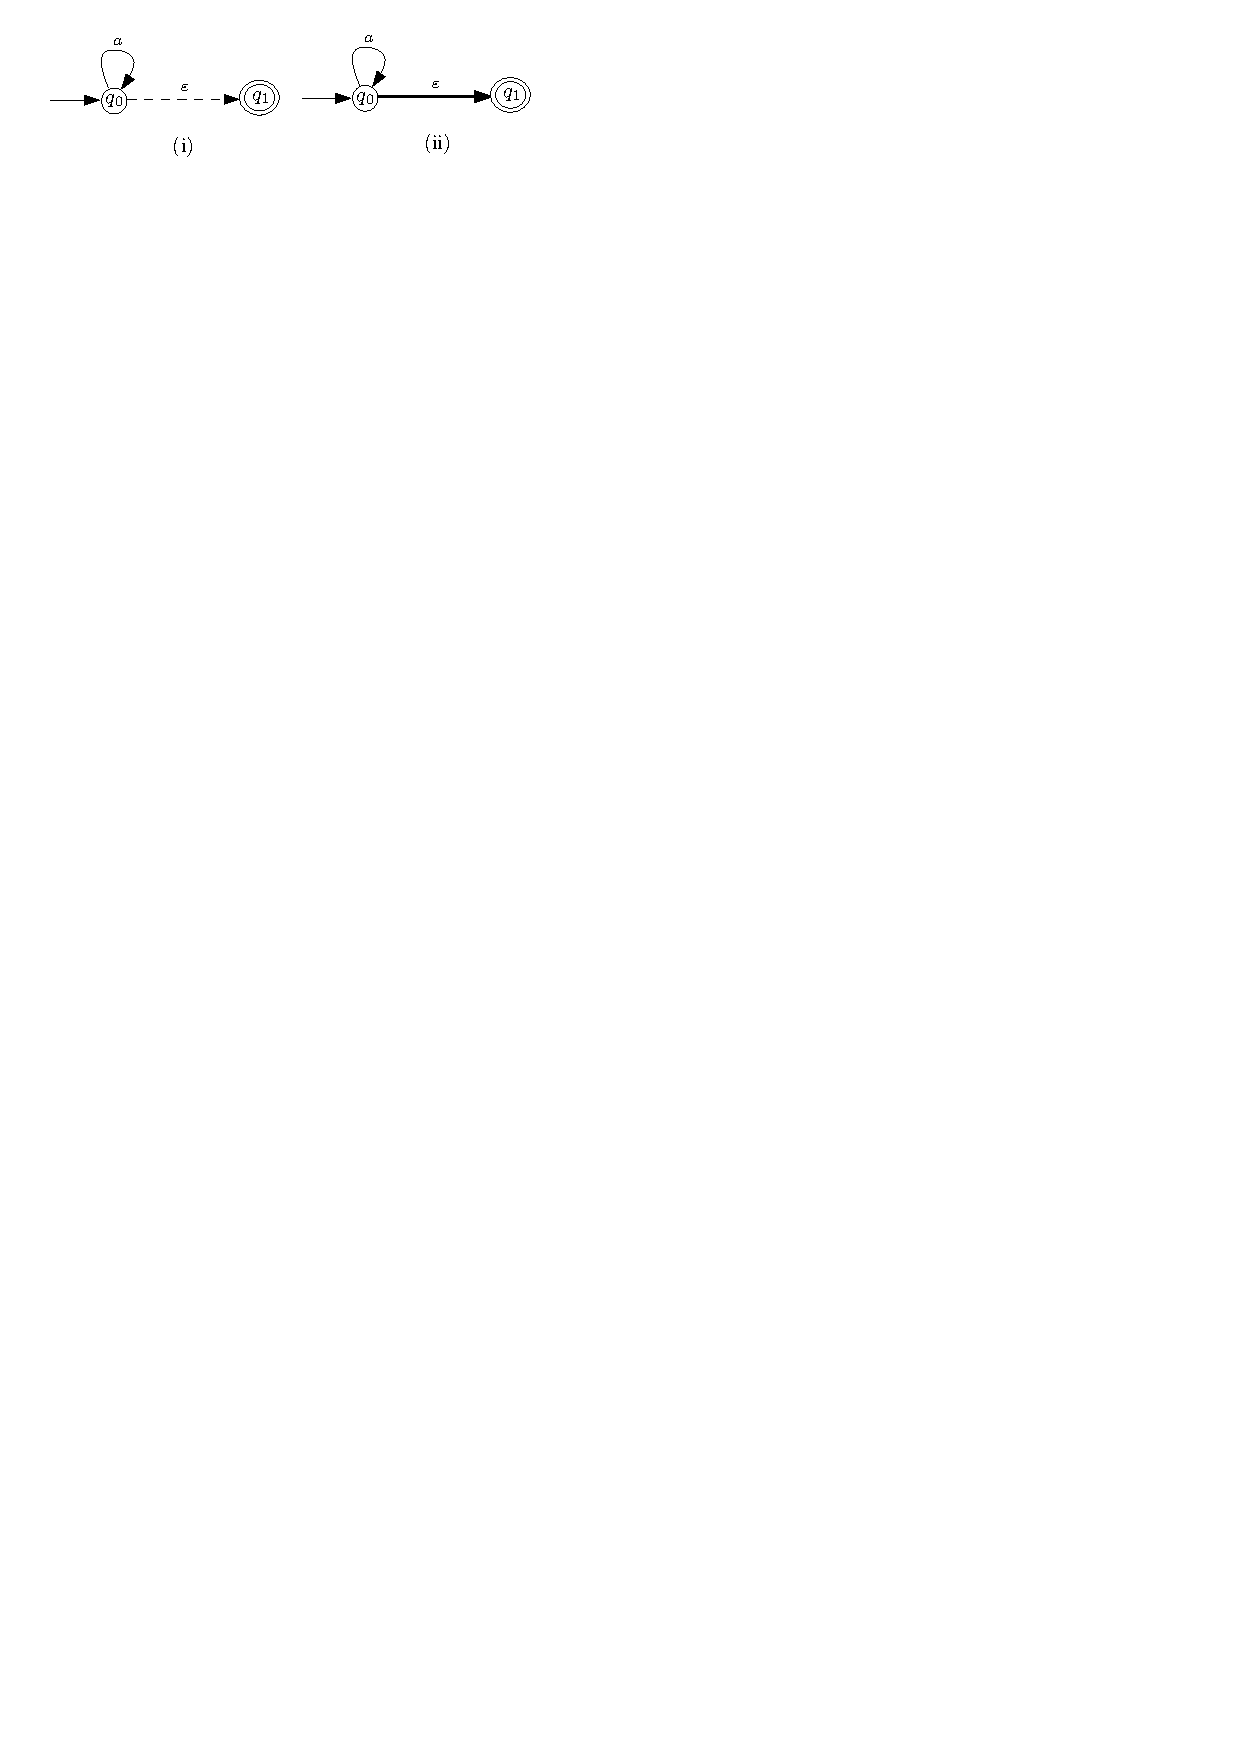
\includegraphics[scale=0.8]{pfa.pdf}
\caption{The PFAs for $a^\ast$ and $a^{\ast?}$}
\label{fig-pfa}
\end{figure}

\end{example}

%\begin{remark}
%Remark that PFAs in Definition~\ref{def-pfa} are different from pNFAs in \cite{BM17} in the sense that the state set in a pNFA is partitioned into two disjoint subsets and the non-$\varepsilon$-transitions are deterministic, while this is not the case in PFAs. Therefore, PFAs are slightly more flexible than pNFAs in \cite{BM17}. We choose this definition of PFAs as a more natural extension of FAs. 
%\end{remark}

The priorities of PFAs are used to model the eager and greedy semantics of $\regexp$, as we shall see in Section~\ref{construction:pnfa}.


%\paragraph{Prioritized streaming string transducers.}

We then introduce prioritized streaming string transducers, a new class of transducers that combine prioritized transducers \cite{BM17} %which combines the expressive power of 
and streaming string transducers \cite{AC10,AD11}.
  
\begin{definition}[Prioritized Streaming String Transducers]
A \emph{prioritized streaming string transducer} (PSST) is a tuple $\psst = (Q, \Sigma, X, \delta, \tau, E, q_0, F)$, where $Q$ a
finite set of states, $\Sigma$ is the input and output alphabet, $X$ is a finite set of variables, $\delta \in Q \times \Sigma \rightarrow \overline{Q}$, $\tau \in Q \rightarrow \overline{Q} \times \overline{Q}$, $E$ is a partial function from $Q \times \Sigma^\varepsilon \times
  Q$ to $X \rightarrow (X \cup \Sigma)^{\ast}$, i.e. the set of assignments,
   $q_0 \in Q$ is the initial state, and $F$ is a partial function
  from $Q$ to $(X \cup \Sigma)^{\ast}$.

A run of $\psst$ on a string $w$ is a sequence $q_0 \sigma_1 s_1 q_1 \ldots \sigma_m s_m q_m$ such that
\begin{itemize}
%\item $q_m \in F$,
%
\item for each $i \in [m]$, 
\begin{itemize}
\item either $\sigma_i \in \Sigma$, $q_i \in \delta (q_{i-1}, \sigma_i)$, and $s_i = E (q_{i - 1}, \sigma_i, q_i)$, 
\item or $\sigma_i = \varepsilon$, $q_i \in \tau(q_{i-1})$ and $s_i = E (q_{i - 1}, \varepsilon, q_i)$,
\end{itemize}

%\item for every subsequence $q_i \sigma_{i+1} s_{i+1} q_{i+1} \ldots \sigma_{j} s_j q_j$ such that  $i < j$ and $\sigma_{i+1} = \cdots = \sigma_j = \varepsilon$, it holds that $q_i, \ldots, q_j$ are mutually distinct. (Intuitively, loops of $\varepsilon$-transitions are forbidden.) 
\item for every subsequence $q_i \sigma_{i+1} s_{i+1} q_{i+1} \ldots \sigma_{j} s_j q_j$ such that  $i < j$ and $\sigma_{i+1} = \cdots = \sigma_j = \varepsilon$,  it holds that for every $k, l: i \le k < l < j$, $(q_k, q_{k+1}) \neq (q_l, q_{l+1})$.
\end{itemize}

%A run of $\psst$ is the sequence $q_0 \sigma_1 s_1 q_1 \ldots \sigma_m s_m q_m$, where $F (q_m)$ is defined and for each $i \in [m], q_i \in \delta (q_{i-1}, \sigma_i)$ and $s_i = E (q_{i - 1}, \sigma_i, q_i)$. 
For any pair of runs $p = q_0 \sigma_1 s_1 \ldots \sigma_m s_m q_m$ and $p' = q_0 \sigma'_1
  s_1' \ldots \sigma'_n s_n' q_n'$ such that $\sigma_1 \ldots \sigma_m = \sigma'_1 \ldots \sigma'_n$, the definition that $p$ is of a higher priority over
  $p'$ is similar to PFAs.
  % $p \neq p'$ and, for the smallest index $j$ with $q_j \neq q_j'$,
 % $\delta (q_{j - 1}, \sigma_j) = \ldots q_j \ldots q_j' \ldots$
  
An accepting run of $\psst$ on an input $w$ is a run of $\psst$ on $w$ of the highest priority, say $q_0 \sigma_1 s_1 \ldots \sigma_m s_m q_m$, such that $F(q_m)$ is defined. The output of $\psst$ on $w$, denoted by $\psst(w)$, is defined as $\eta_m(F(q_m))$, where $\eta_0(x) = \varepsilon$ for each $x \in X$, and $\eta_{i}(x) = \eta_{i-1}(s_{i}(x))$ for every $1 \le i \le m$ and $x \in X$. Note that here we abuse the notation  $\eta_m(F(q_m))$ and $\eta_{i-1}(s_{i}(x))$ by taking a function $\eta$ from $X$ to $\Sigma^*$ as a function from $(X \cup \Sigma)^*$ to $\Sigma^*$, which maps each $\sigma \in \Sigma$ to $\sigma$ and each $x \in X$ to $\eta(x)$. If there is no accepting run of $\psst$ on $w$, then $\psst(w) = \bot$, namely, the output of $\psst$ on $w$ is undefined. The string relation defined by $\psst$, denoted by $\cR_\psst$,  is $\{(w, \psst(w)) \mid w \in \Sigma^\ast, \psst(w) \neq \bot\}$.
\end{definition}

\begin{example}
The PSST $\cT_{\sf nameReg}=(Q, \Sigma, X, \delta, \tau, E,  q_{0}, F)$ mentioned in Section~\ref{sec:mot} is illustrated in Figure~\ref{fig-psst-exmp}, where $Q = \{q_0, \dots, q_{24}\}$, $X= \{x_1, x_2, x_3, x_4\}$ with $x_1, x_2, x_3$ recording the matches of the 1st, 2nd, 3rd capturing group, and $x_4$ recording the string after the replacements, $F(q_{24}) = x_4$ denotes the final output, and $\delta, \tau, E$ are illustrated by the edges, where the dashed edges denote the $\varepsilon$-transitions of lower priorities than the non-$\varepsilon$-transitions and the symbol $\ell$ is used to denote the currently scanned input letter. For instance, $\delta(q_3, \backslash\mbox{s}) = (q_3)$, $\delta(q_3, \ell) = ()$ for every $\ell \in \Sigma \setminus \{\backslash\mbox{s}\}$, $\tau(q_3) = ((); (q_4))$, and $E(q_3, \backslash\mbox{s}, q_3)(x_1) = x_1 \backslash s$. Since the $\varepsilon$-transition has lower priority than the $\backslash\mbox{s}$-transition at the state $q_3$, whenever the currently scanned letter is $\backslash$s at $q_3$,  $\cT_{\sf nameReg}$ will choose to go to $q_3$ greedily, until there is no more $\backslash$s. (In this case, it has to choose the $\epsilon$-transition and goes to $q_4$.) Note that the identity assignments, e.g. $E(q_3, \backslash\mbox{s}, q_3)(x') = x'$ for $x' \in \{x_2, x_3, x_4\}$, are omitted in Figure~\ref{fig-psst-exmp}, for readability. 
%From $\delta(q_4, \backslash s) = q_5q_{6}$, we know that $q_5$ is prior to $q_6$. 
%Therefore, whenever $\cT_{\sf nameReg}$ reads $\backslash$s at the state $q_3$,  it will choose to go the state $q_5$ greedily, unless this choice would lead to the nonacceptance (in this case, $q_6$ will be chosen). 
\begin{figure*}[ht]
\centering
%\rule{\linewidth}{0cm}
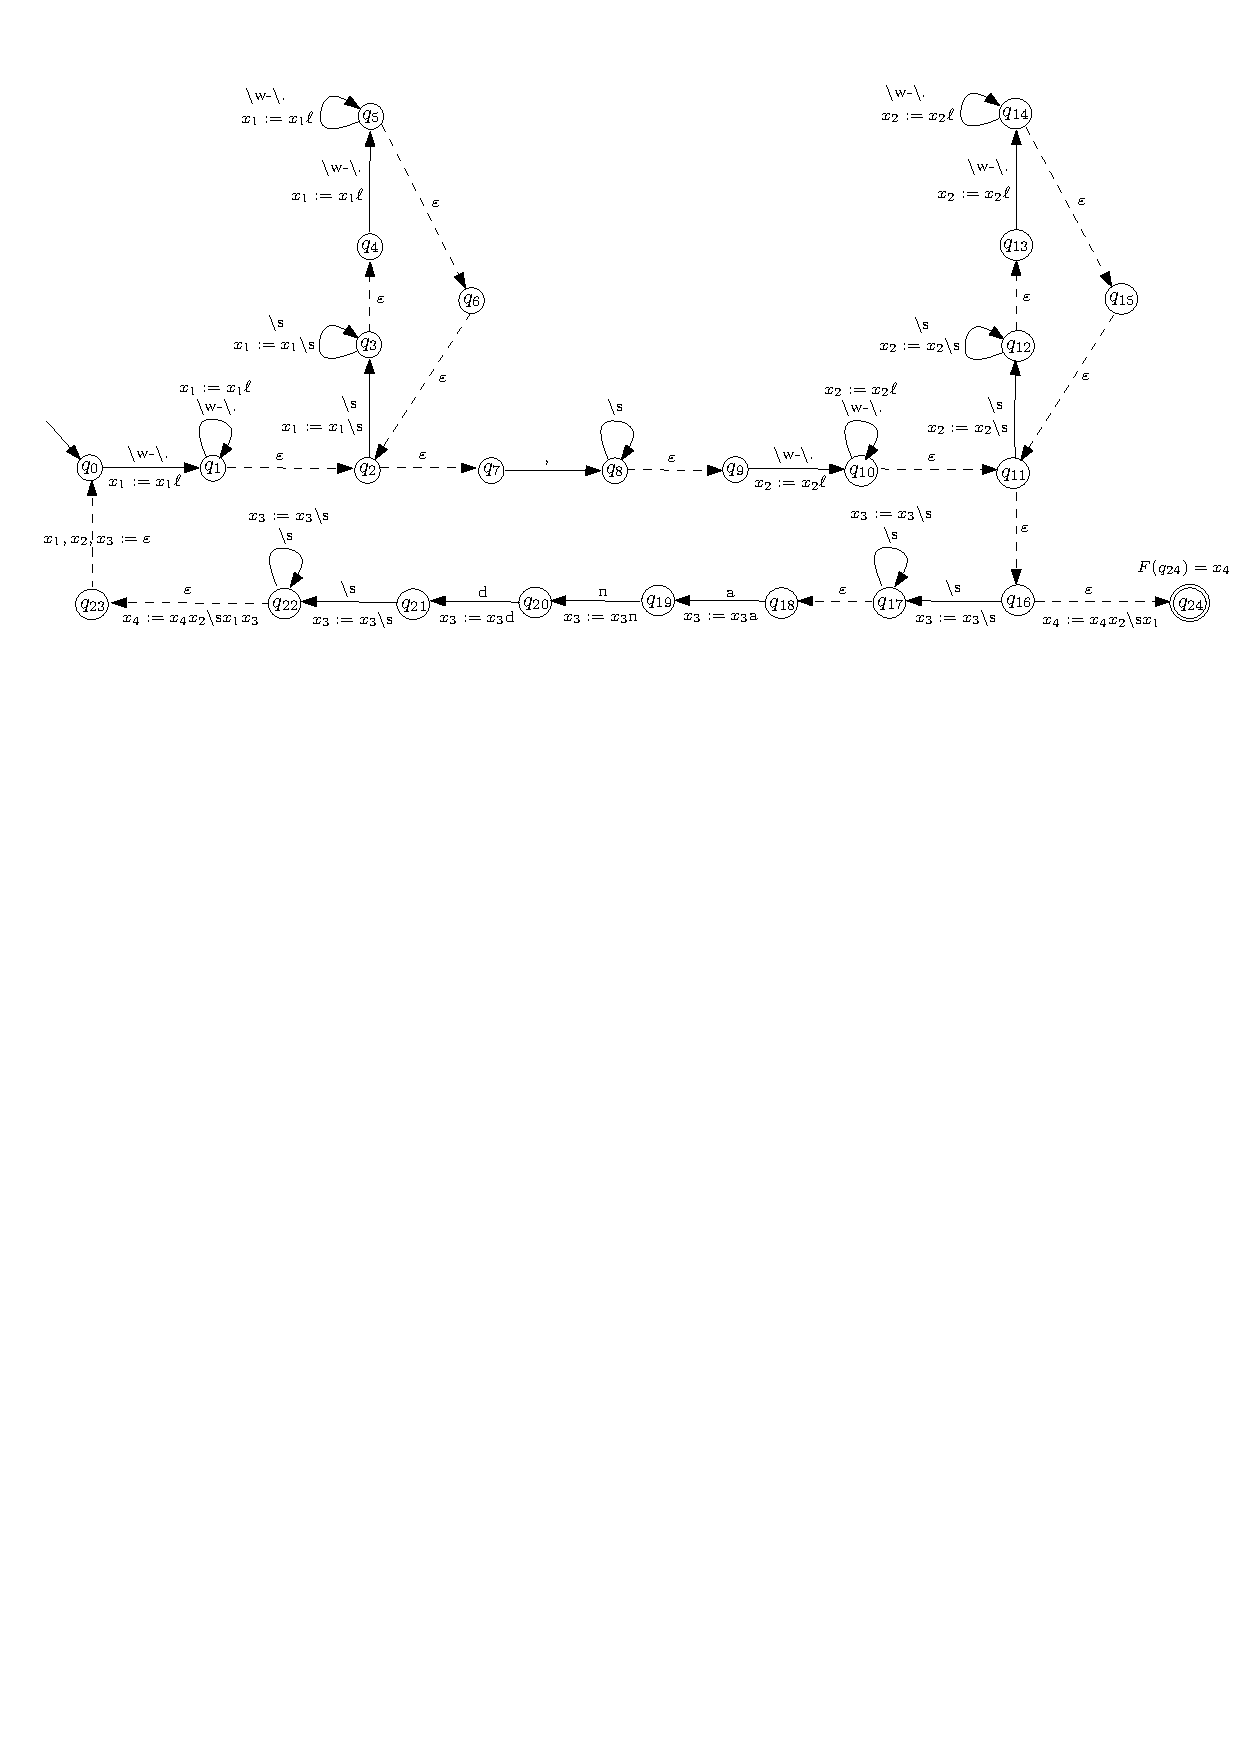
\includegraphics[scale=0.8]{psst-epsilon-exmp.pdf}
\caption{The PSST $\cT_{\sf nameReg}$}
\label{fig-psst-exmp}
\end{figure*}
\end{example}

  
%  $\tmop{Out} (r) =
%  s_{\varepsilon} \circ s_1 \circ s_2 \ldots s_n \circ F (q_n)$ where
%  $s_{\varepsilon}$ is the empty substitution which maps all variables to
%  $\varepsilon$.
  
\begin{definition}[Pre-image]
For a string relation $R \subseteq \Sigma^* \times \Sigma^*$ and $L \subseteq \Sigma^*$, we define the \emph{pre-image} of $L$ under $R$ as $R^{-1}(L):=\{w \in \Sigma^* \mid \exists w'.\ w' \in L \mbox{ and } (w, w') \in R\}$. 
\end{definition}
 
\begin{theorem}[Pre-image of \PSST{}]
  \label{theorem:psst_preimage}
  Given a \PSST{} $\psst = (Q_T, \Sigma$, $X, \delta_T, \tau_T, E_T,  q_{0, T}, F_T)$ and an \FA{} $\Aut
  = (Q_A, \Sigma, \delta_A, q_{0, A}, F_A)$, we can compute an \FA{} $\cB = (Q_B,
  \Sigma, \delta_B, q_{0, B}, F_B)$ in exponential time  such that $\Lang(\cB) = \cR^{-1}_{\cT}(\Lang(\Aut))$.
\end{theorem}

\tl{another way is to first define B as a PFA, could make the construction a bit modular?}\zhilin{Add a counter example for this natural idea.}
 
Let $\psst = (Q_T, \Sigma$, $X, \delta_T, \tau_T, E_T,  q_{0, T}, F_T)$ be a \PSST{}  and $\Aut
  = (Q_A, \Sigma, \delta_A, q_{0, A}, F_A)$ be an \FA{}. Without loss of generality, we assume that $\Aut$ contains no $\varepsilon$-transitions. 

To illustrate the intuition of the FA construction, let us start with the following natural idea of firstly constructing a PFA $\cB$ for the pre-image: $\cB$ simulates the run of $\psst$ on $w$, and, for each $x \in X$, records an $\Aut$-abstraction of the string stored in $x$, that is, the set of state pairs $(p, q) \in Q_A \times Q_A$ such that starting from $p$, $\Aut$ can reach $q$ after reading the string stored in $x$. Specifically, the states of $\cB$ are of the form $(q, \rho)$ with $q \in Q$ and $\rho \in (\cP(Q_A \times Q_A ))^{X}$. Moreover, the priorities of $\cB$ inherit those of $\Aut$. The PFA $\cB$ is then transformed to an equivalent FA by simply dropping all priorities. We refer to this FA as $\cB'$.

Nevertheless, it turns out that this construction method is flawed: A string $w$ is in $\cR^{-1}_{\cT}(\Lang(\Aut))$ iff the (unique) accepting run of $\cT$ on $w$ produces an output $w'$ that is accepted by $\Aut$. However, a string $w$ is accepted by $\cB'$ iff there is a run of $\cT$ on $w$, not necessarily of the highest priority, producing an output $w'$ that is accepted by $\Aut$. The following example illustrates the flaw of the construction above.

\begin{example}
\label{pre-image-count-examp}
Let $\cT$ be the PSST and $\cA$ be the FA in Figure~\ref{fig-pre-image-count-exmp}, that is, 
\begin{itemize}
\item $\cT=(\{q_0, q_1, q_2\}, \{a,b,c\}, \{x_0\}, \delta_T, \tau_T, E_T, q_0, F_T)$, where $\delta_T(q_0, \sigma) = (q_0)$, $\delta_T(q_1, a) = (q_1)$, $\delta_T(q_2, \sigma) = (q_2)$, $\tau_T(q_0) = ((q_1); ())$, $\tau_T(q_1)=((q_0, q_2);())$, and $\tau_T(q_2)= ((); ())$, $E_T(q_0, \sigma, q_0) (x_0) = x_0 \sigma$, $E_T(q_1, \varepsilon, q_0) (x_0) = x_0 c$, $E_T(q_1, \varepsilon, q_2) (x_0) = x_0 c$, $E_T(q_2, \sigma, q_2) (x_0) = x_0 \sigma$, for $\sigma \in\{ a, b\}$. Moreover, $F_T(q_2)= x_0$;
%
\item $\cA = (\{p_0\}, \{a,b,c\}, \delta_A, p_0, \{p_0\})$, where $\delta_A$ = $\{(p_0, \sigma, p_0)$ $\mid \sigma = b, c\}$.
\end{itemize}

Let us consider $w = a$. The accepting run of $\cT$ on $w$ is $q_0 \xrightarrow{\varepsilon} q_1 \xrightarrow[x_0:=x_0c]{\varepsilon} q_0 \xrightarrow[x_0:=x_0a]{a} q_0 \xrightarrow{\varepsilon} q_1 \xrightarrow[x_0:=x_0c]{\varepsilon} q_2$, producing an output $cac \not \in \Lang(\cA)$. Therefore, $a \not \in \cR_\cT^{-1}(\Lang(\cA))$. Nevertheless, if we consider the FA $\cB'$ constructed from $\cT$ and $\cA$,  it turns out that $\cB'$ does accept $w$, witnessed by the run $(q_0, \{(p_0,p_0)\}) \xrightarrow{\varepsilon} (q_1, \{(p_0,p_0)\}) \xrightarrow{a} (q_1, \{(p_0, p_0)\}) \xrightarrow{\varepsilon}  (q_2, \{(p_0, p_0)\})$. On the other hand, the run of $\cB'$ corresponding to the accepting run of $\cT$ on $w$, i.e. $(q_0, \{(p_0,p_0)\}) \xrightarrow{\varepsilon} (q_1, \{(p_0,p_0)\}) \xrightarrow{\varepsilon} (q_0, \{(p_0, p_0)\}) \xrightarrow{a}  (q_0, \emptyset) \xrightarrow{\varepsilon} (q_1, \emptyset) \xrightarrow{\varepsilon} (q_2, \emptyset)$, is not accepting, where $\{(p_0,p_0)\}$ and $\emptyset$ are the $\cA$-abstractions of $x_0$.
\end{example}

\begin{figure}[ht]
\centering
%\rule{\linewidth}{0cm}
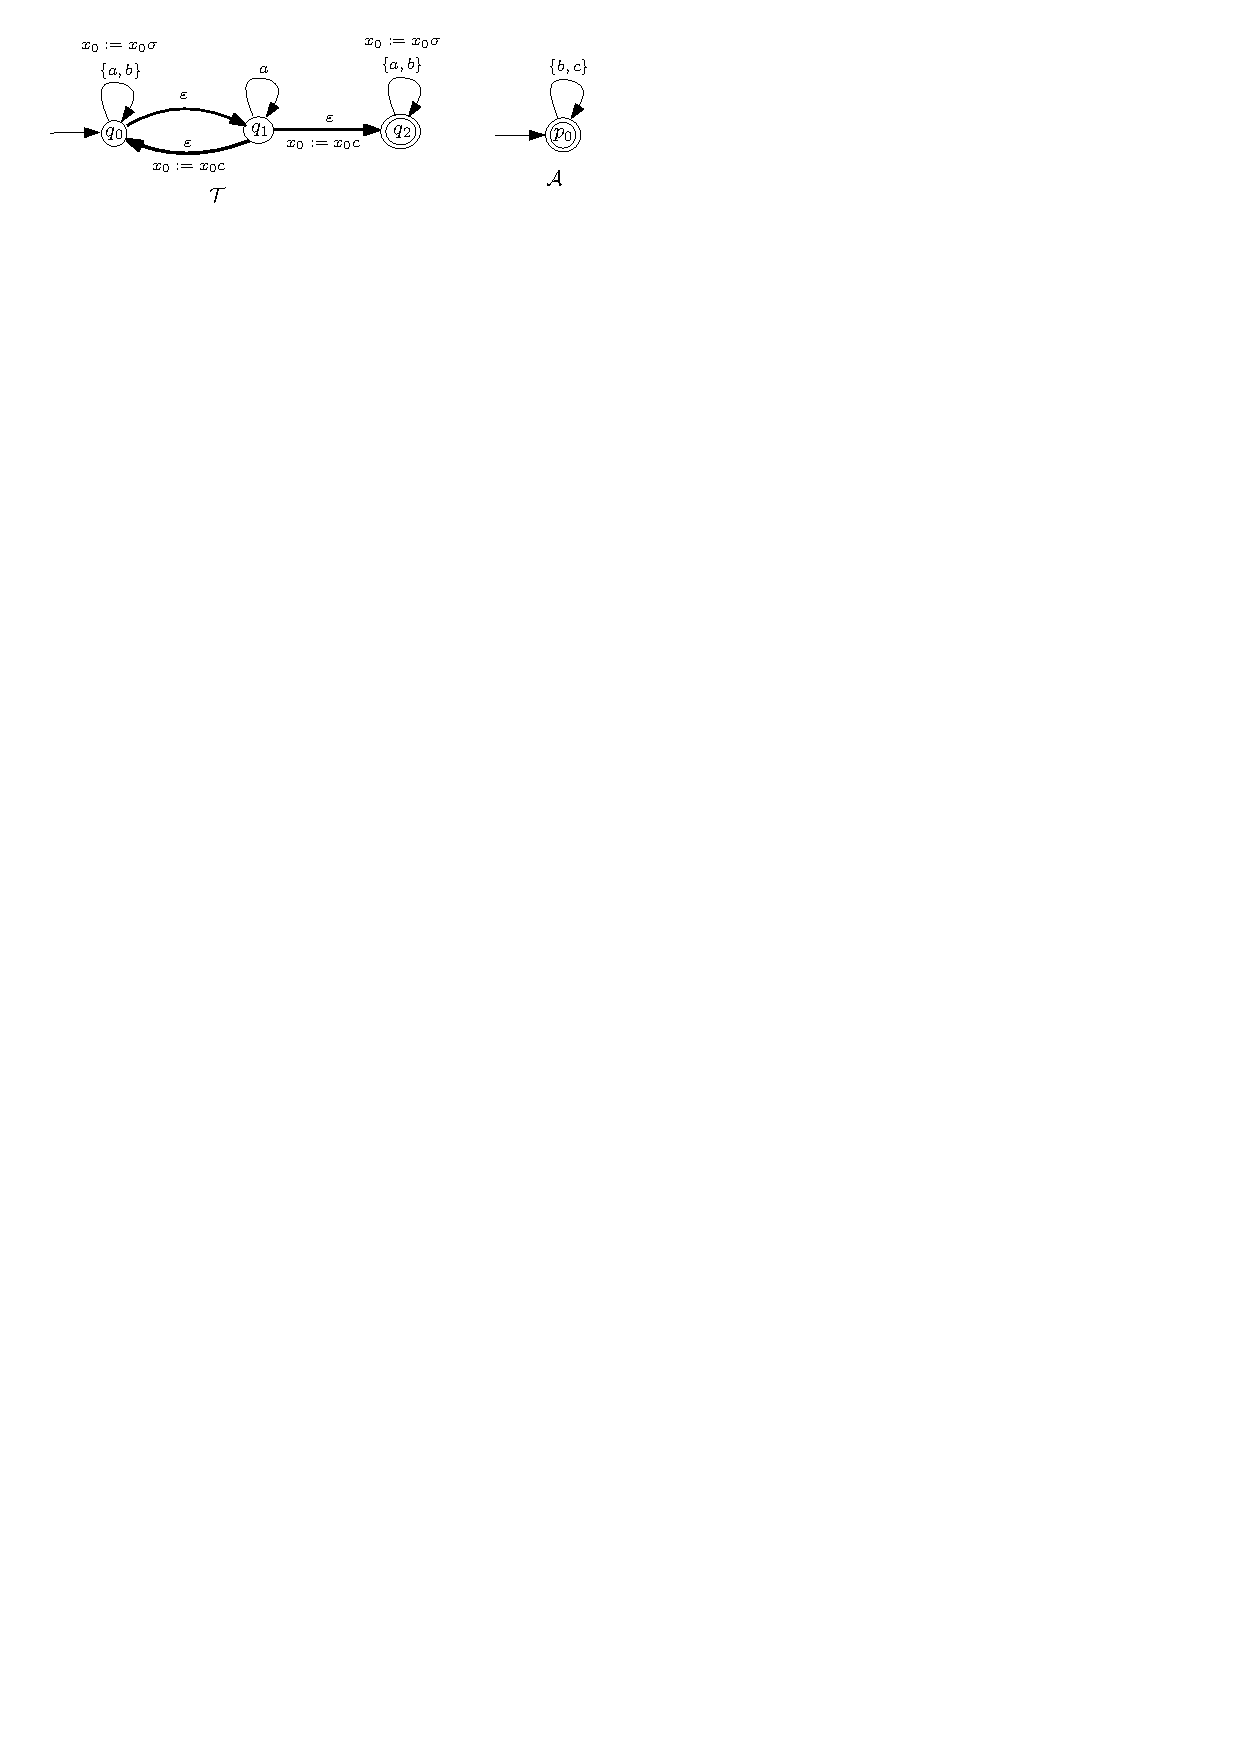
\includegraphics[scale=0.8]{pre-image-counter-example.pdf}
\caption{A counterexample to disprove the flawed pre-image construction method}
\label{fig-pre-image-count-exmp}
\end{figure}

\begin{proof}[Proof of Theorem~\ref{theorem:psst_preimage}]
Let $\psst = (Q_T, \Sigma$, $X, \delta_T, \tau_T, E_T,  q_{0, T}, F_T)$ be a \PSST{} and $\Aut
  = (Q_A, \Sigma, \delta_A, q_{0, A}, F_A)$ be an \FA{}. For convenience, we use $\cE(\tau_T)$ to denote $\{(q, q') \mid q' \in \tau_T(q)\}$.

Our goal is to construct a FA $\cB$ that simulates the run of $\psst$ on $w$, and, for each $x \in X$, records an $\Aut$-abstraction of the string stored in $x$, that is, the set of state pairs $(p, q) \in Q_A \times Q_A$ such that starting from $p$, $\Aut$ can reach $q$ after reading the string stored in $x$. To simulate the runs of $\psst$, it is necessary to record all the states accessible from a run of higher priority to ensure the current run is an accepting run of $\psst$ of highest priority. Moreover, $\cB$ also remembers the set of $\varepsilon$-transitions of $\cT$ after the latest non-$\varepsilon$-transition to ensure that no transition occurs twice in a sequence of $\varepsilon$-transitions of $\cT$.

Specifically, each state of $\cB$ is of the form $(q, \rho, \Lambda, S)$, where $q \in Q_T$, $\rho \in (\cP(Q_A \times Q_A ))^{X}$, $\Lambda \subseteq \cE(\tau_T)$, and $S \subseteq Q_T$. Note that when recording in $S$ all the states accessible from a run of higher priority, we do not take the non-repetition of $\varepsilon$-transitions into consideration since if a state is reachable by a sequence of $\varepsilon$-transitions where some $\varepsilon$-transitions are repeated, then there exists also a sequence of non-repeated $\varepsilon$-transitions reaching the state. Moreover, when simulating a $\sigma$-transition of $\cT$ (where $\sigma \in \Sigma$) at a state $(q, \rho, \Lambda, S)$, $\cB$ should saturate the states in $S$ by $\varepsilon$-transitions, that is, compute the set of states that are reachable from the states in $S$ by a sequence of $\varepsilon$-transitions, then apply a $\sigma$-transition to them. For technical reasons, when constructing $\cB$, we assume that this saturation happens when a state is added to $S$ for the first time. Therefore, at a state $(q, \rho, \Lambda, S)$, all the states reachable from the states in $S$ by sequences of $\varepsilon$-transitions in $\cT$ have already been in $S$.
%ready for taking non-$\varepsilon$ transitions, 

Before the construction of $\cB$, we introduce some notations.
\begin{itemize}
\item For $S \subseteq Q_T$, $\delta^{(ip)}_T(S, a) = \{q'_1 \mid \exists q_1 \in S, q'_1 \in \delta_T(q_1, a)\}$.
%
\item For $q \in Q_T$,  if $\tau_T(q) = (P_1, P_2)$, then $\tau^{(ip)}_T(\{q\})=S$ such that $S = P_1 \cup P_2$. 
Moreover, for $S \subseteq Q_T$, we define $\tau^{(ip)}_T(S) = \bigcup \limits_{q \in S} \tau^{(ip)}_T(\{q\})$. We also use $\big(\tau^{(ip)}_T\big)^\ast$ to denote the $\varepsilon$-closure of $\cT$, namely, $\big(\tau^{(ip)}_T\big)^\ast(S) = \bigcup \limits_{n \in \Nat} \big(\tau^{(ip)}_T\big)^{n}(S)$, where $\big(\tau^{(ip)}_T\big)^{0}(S) = S$, and for $n \in \Nat$, $\big(\tau^{(ip)}_T\big)^{n+1}(S) = \tau^{(ip)}_T\big(\big(\tau^{(ip)}_T\big)^{n}(S)\big)$. 
%
\item For $S \subseteq Q_T$ and $\Lambda \subseteq  \cE(\tau_T)$, we use $\big(\tau^{(ip)}_T \backslash \Lambda\big)^\ast(S)$ to denote the set of states reachable from $S$ by sequences of $\varepsilon$-transitions where {\it no} transitions $(q, \varepsilon, q')$ such that $(q, q') \in \Lambda$ are used.
%
%We also use $(\tau^{(ip)}_T)^\ast$ to denote the reflexive transitive closure of $\tau^{(ip)}_T$. \tl{here $(\tau^{(ip)}_T)$ is defined as a function... you mean function composition?}
%\zhilei{I think we can just use the term 'epsilon closure' here?}
%\item For $\sigma \in \Sigma$ and $S \subseteq Q_T$,  we use $\tau^+_T[a, S]$ to denote the set of states that can be obtained from 
% 
\item For $\rho \in (\cP(Q_A \times Q_A ))^{X}$ and $s \in X \rightarrow (X \cup \Sigma)^{\ast}$, we use $s(\rho)$ to denote $\rho'$ that is obtained from $\rho$ as follows: For each $x \in X$, if $s(x) = \varepsilon$, then $\rho'(x) = \{(p, p) \mid p \in Q_A\}$, otherwise, let $s(x) = b_1 \cdots b_\ell$ with $b_i \in \Sigma \cup X$ for each $i \in [\ell]$, then $\rho'(x) = \theta_1 \circ \cdots \circ \theta_\ell$, where $\theta_i = \delta^{(b_i)}_A$ if $b_i \in \Sigma$, and $\theta_i = \rho(b_i)$ otherwise.
\end{itemize}

We are ready to present the formal construction of $\cB =  (Q_B$, $\Sigma$, $\delta_B$, $q_{0, B}, F_B)$. 
\begin{itemize}
\item $Q_B = Q_T \times (\cP(Q_A \times Q_A ))^{X} \times \cP(\cE(\tau_T)) \times \cP(Q_T)$, 
%(Intuitively, the letter $\sigma$ in $(q, \sigma, \rho, S) \in Q_B$ means the next letter to be read at $q$, with $\bot$ represents the end of the input.)

\item $q_{0, B} = (q_{0,T}, \rho_{\varepsilon}, \emptyset, \emptyset)$ where $\rho_{\varepsilon} (x) = \{(q, q) \mid q \in Q\}$ for each $x \in X$,

\item $\delta_{B}$ comprises 
\begin{itemize}
%\item the tuples $(q'_0, \varepsilon, ((q_{0,T},\sigma), \rho_{\varepsilon}, \emptyset))$ where $\sigma \in \Sigma$, $\rho_{\varepsilon} (x) = \{(q, q) \mid q \in Q\}$ for each $x \in X$, 
%
\item the tuples $((q, \rho, \Lambda, S), \sigma, (q_i, \rho', \Lambda', S'))$ such that  
%there exists $s \in \left((X \cup \Sigma\right)^*)^X)$ satisfying
\begin{itemize}
\item $\sigma \in \Sigma$, 
%$\sigma' \in \Sigma \cup \{\bot\}$, 
%
\item $\delta_T (q, \sigma) = (q_1, \ldots, q_i, \ldots, q_m)$, 
%
\item $s = E(q, \sigma, q_i)$, 
%
\item $\rho' = s(\rho)$,
%
\item $\Lambda' = \emptyset$, (Intuitively, $\Lambda$ is reset.)
%
\item let $\tau_T(q) = (P_1, P_2)$, then $S' = \big(\tau^{(ip)}_T\big)^\ast\big(\{ q_1$, $\ldots$, $q_{i - 1} \} \cup \delta^{(ip)}_T\big(S \cup \big(\tau^{(ip)}_T \setminus \Lambda\big)^\ast(P'_1), \sigma\big)\big)$, where $P'_1 = \{q' \in P_1 \mid (q, q') \not \in \Lambda\}$;  (Note that according to the semantics of PSSTs, when computing the set of states reachable from $q$ through an $\varepsilon$-transition to some $q' \in P_1$ first and a sequence of $\varepsilon$-transitions starting from $q'$ next, the transitions $(q'', \varepsilon, q''')$ with $(q'', q''') \in \Lambda$ should be excluded. )
%(Intuitively, we assume that $S$ is the current set of states ready for taking non-$\varepsilon$-transitions and has already included the states belonging to its $\varepsilon$-closure, moreover, $S'$ is the $\varepsilon$-closure of the set of states reached after taking a $\sigma$-transition.)
%the set of states that can be reached from $S \cup (\tau^{(ip)}_T)^\ast(P_1)$ by a sequence of $\varepsilon$-transitions, followed by a $\sigma$-transition, 
%more precisely, suppose $(\tau^{(ip)}_T)^\ast(S \cup P_1) = S''$, then $S' =  \delta^{(ip)}_T(S'', \sigma)$ $\cup$ $\{ q_1$, $\ldots$, $q_{i - 1} \}$; 
%
%$\rho'(x) = \theta_\ell$ such that $\theta_0 = \{(p,p) \mid p \in Q_A\}$, and for each $i \in [\ell]$, if $b_i \in \Sigma$, then $\theta_i = \{(p, p') \mid (p, p'') \in \theta_{i-1}, (p'', b_i, p') \in \delta_A \mbox{ for some } p''\}$, otherwise, $\theta_i = \theta_{i-1} \cdot \rho(x)$. 
\end{itemize}
%
\item the tuples $((q, \rho, \Lambda, S), \varepsilon, (q_i, \rho', \Lambda', S'))$ such that 
%there exists $s \in \left((X \cup \Sigma\right)^*)^X$ satisfying
\begin{itemize}
%, $\sigma' \in \Sigma \cup \{\bot\}$, 
%
\item $\tau_T(q) = ((q_1, \ldots, q_i, \ldots, q_m); \cdots)$, 
%
\item $(q, q_i) \not \in \Lambda$,

\item $s = E(q, \varepsilon, q_i)$, 
%
\item $\rho' = s(\rho)$,
%
\item $\Lambda' = \Lambda \cup \{(q, q_i)\}$, 
%
\item $S' =  S \cup \big(\tau^{(ip)}_T \backslash \Lambda \big)^\ast(\{ q_j \mid j \in [i-1], (q, q_j) \not \in \Lambda \})$;
%
%$\rho'(x) = \theta_\ell$ such that $\theta_0 = \{(p,p) \mid p \in Q_A\}$, and for each $i \in [\ell]$, if $b_i \in \Sigma$, then $\theta_i = \{(p, p') \mid (p, p'') \in \theta_{i-1}, (p'', b_i, p') \in \delta_A \mbox{ for some } p''\}$, otherwise, $\theta_i = \theta_{i-1} \cdot \rho(x)$. 
\end{itemize}
%

\item the tuples $((q, \rho, \Lambda, S), \varepsilon, (q_i, \rho', \Lambda', S'))$ such that 
%there exists $s \in \left((X \cup \Sigma\right)^*)^X$ satisfying
\begin{itemize}
%\item $\sigma \in \Sigma$, 
%$\sigma' \in \Sigma \cup \{\bot\}$, 
%
\item $\tau_T (q) = ((q'_1, \ldots, q'_n); (q_1, \ldots, q_i, \ldots, q_m))$, 
%
\item $(q, q_i) \not \in \Lambda$,
%
\item $s = E(q, \varepsilon, q_i)$,
%
\item $\rho' = s(\rho)$,
%
\item $\Lambda' = \Lambda \cup \{(q, q_i)\}$, 
%
\item $S' = S \cup \{q\} \cup \big(\tau^{(ip)}_T \backslash \Lambda \big)^\ast\big(\big\{q'_j \mid j \in [n], (q, q'_j) \not \in \Lambda \big\} \cup \big\{q_j \mid j \in [i-1], (q, q_j) \not \in \Lambda \big\} \big)$. (Note that here we include $q$ into $S'$, since the non-$\varepsilon$-transitions out of $q$ have higher priorities than the transition $(q, \varepsilon, q_i)$.)
%
%$\rho'(x) = \theta_\ell$ such that $\theta_0 = \{(p,p) \mid p \in Q_A\}$, and for each $i \in [\ell]$, if $b_i \in \Sigma$, then $\theta_i = \{(p, p') \mid (p, p'') \in \theta_{i-1}, (p'', b_i, p') \in \delta_A \mbox{ for some } p''\}$, otherwise, $\theta_i = \theta_{i-1} \cdot \rho(x)$. 
\end{itemize}
\end{itemize}
\item
Moreover, $F_B$ is the set of states $(q, \rho, \Lambda, S) \in Q_B$ such that
\begin{enumerate}
  \item $F_T (q)$ is defined,
%
  \item for any $q' \in S$, $F_T (q')$ is not defined,
  %
  \item if $F_T(q) = \varepsilon$, then $q_{0, A}  \in F_A$, otherwise, 
let $F_T(q) = b_1 \cdots b_\ell$ with $b_i \in \Sigma \cup X$ for each $i \in [\ell]$, then $(\theta_1 \circ \cdots \circ \theta_\ell) \cap (\{q_{0,A}\} \times F_A) \neq \emptyset$, where for each $i \in [\ell]$, if $b_i \in \Sigma$, then $\theta_i = \delta^{(b_i)}_A$, otherwise, $\theta_i = \rho(b_i)$.
\end{enumerate}
\end{itemize}
\end{proof}

Note that the above construction  does not utilize the so-called \tmtextit{copyless} property \cite{AC10,AD11},
  thus it works for general, or \textit{copyful} \PSST{} \cite{FR17}.

\begin{example}
Figure \ref{fig-psst-preimage-exmp} gives the correct FA $\cB$ encoding $\cR^{-1}_{\cT}(\Lang(\Aut))$ in Example \ref{pre-image-count-examp} using the construction method introduced above. Only those states reachable from the initial state $r_0$ are shown. Table \ref{table:psst-preimage} shows the correspondence between the states in the figure and the states of $\cB$, where $\rho_1(x)=\{(p_0,p_0)\}$ and $\rho_2(x)=\emptyset$.

Note that many states are redundant. For efficiency, we minimize the FA after the construction. See Section \ref{sect:impl} for implementation details.
\end{example}


\begin{figure}[ht]
\centering
%\rule{\linewidth}{0cm}
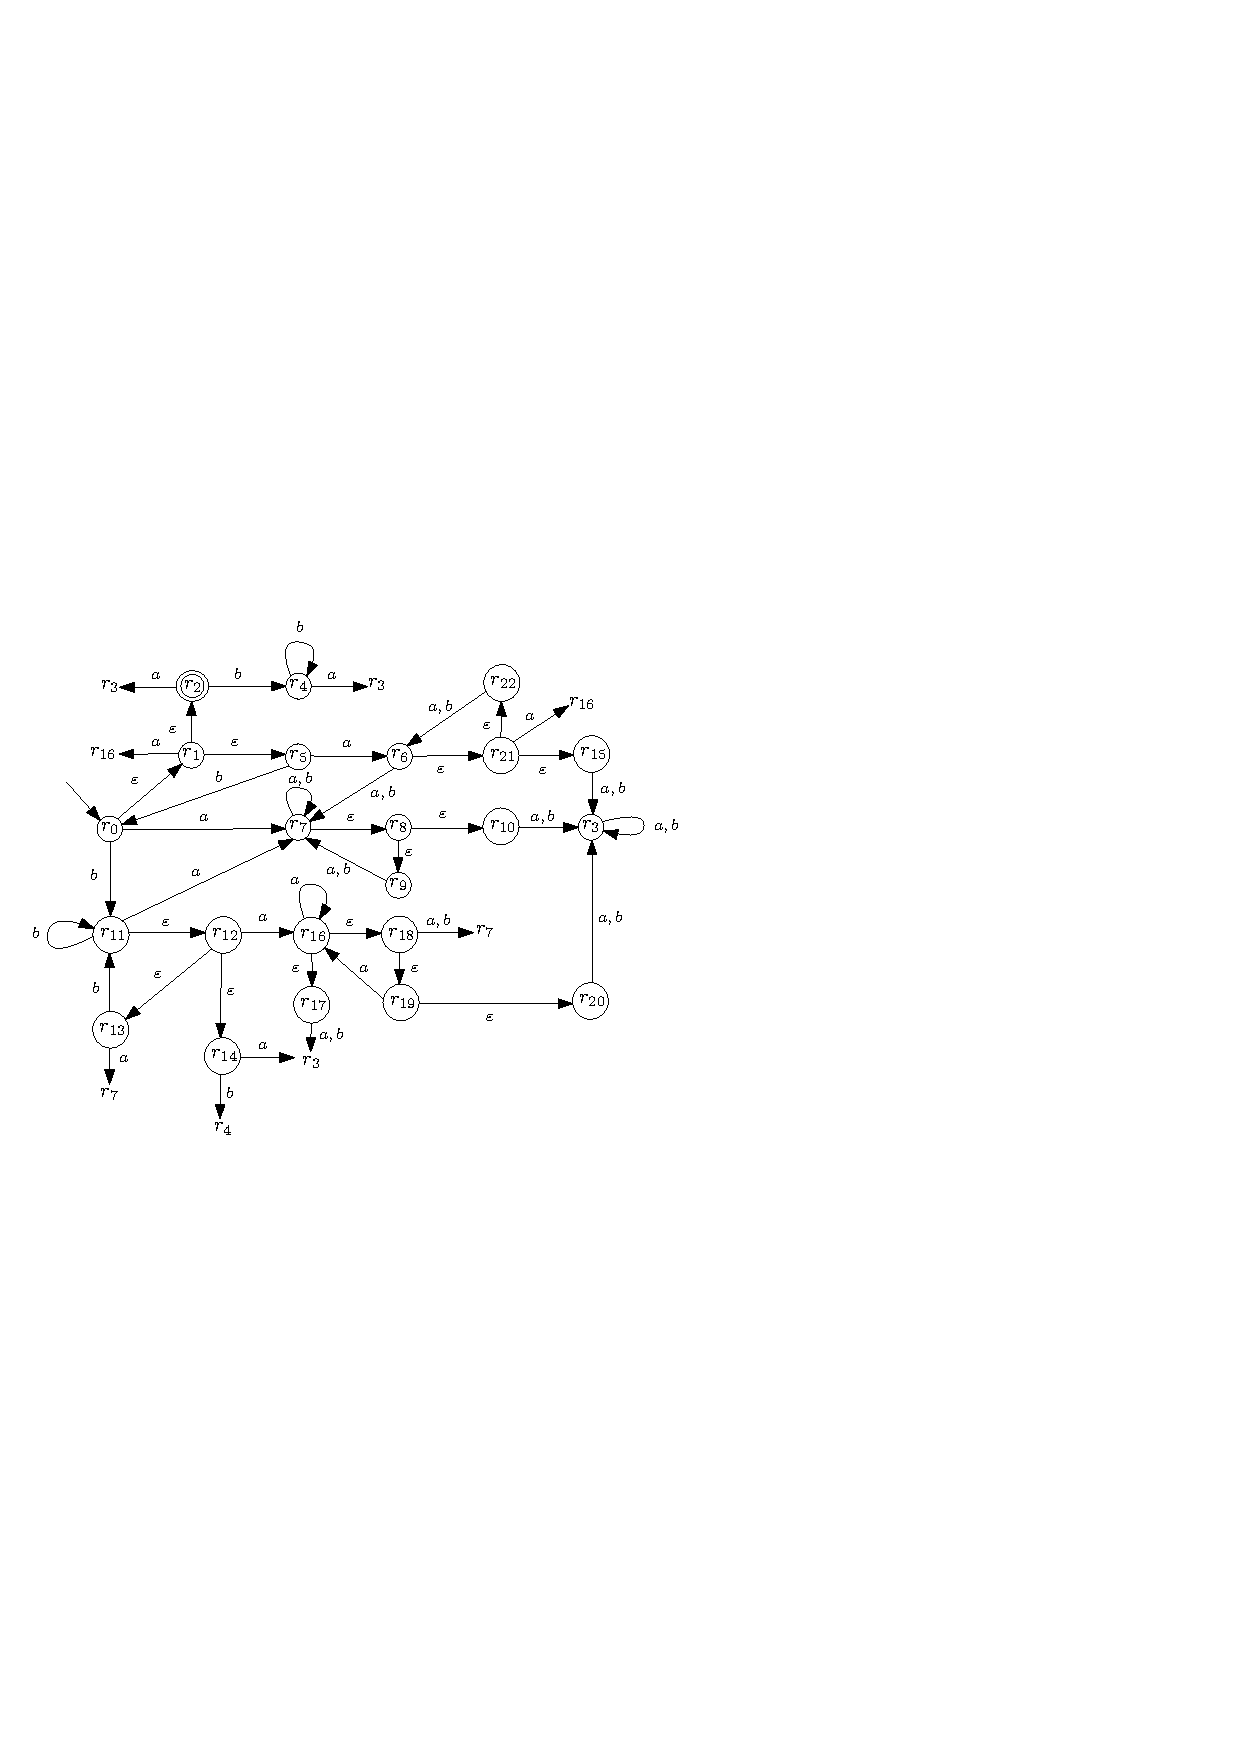
\includegraphics[scale=0.8]{psst-preimage-example.pdf}
\caption{FA $\cB$ that encodes $\cR^{-1}_{\cT}(\Lang(\Aut))$}
\label{fig-psst-preimage-exmp}
\end{figure}

\begin{table}[t]
\centering
\caption{the actual $\cB$ state in Figure 
\label{table:psst-preimage}
\ref{fig-psst-preimage-exmp}}
\begin{tabular}{|c|c|}
    \hline
    Symbol & State of $\cB$\\
    \hline
    $r_0$ & $(q_0, \rho_1, \emptyset, \emptyset)$\\
    \hline
    $r_1$ & $(q_1, \rho_1, \{ (q_0, q_1) \}, \emptyset)$\\
    \hline
    $r_2$ & $(q_2, \rho_1, \{ (q_0, q_1), (q_1, q_2) \}, \{ q_0 \})$\\
    \hline
    $r_3$ & $(q_2, \rho_2, \emptyset, \{ q_0, q_1, q_2 \})$\\
    \hline
    $r_4$ & $(q_2, \rho_1, \emptyset, \{ q_0, q_1, q_2 \})$\\
    \hline
    $r_5$ & $(q_0, \rho_1, \{ (q_0, q_1) (q_1, q_0) \}, \emptyset)$\\
    \hline
    $r_6$ & $(q_0, \rho_2, \emptyset, \emptyset)$\\
    \hline
    $r_7$ & $(q_0, \rho_2, \emptyset, \{ q_0, q_1, q_2 \})$\\
    \hline
    $r_8$ & $(q_1, \rho_2, \{ (q_0, q_1) \}, \{ q_0, q_1, q_2 \})$\\
    \hline
    $r_9$ & $(q_0, \rho_2, \{ (q_0, q_1) (q_1, q_0) \}, \{ q_0, q_1, q_2 \})$\\
    \hline
    $r_{10}$ & $(q_2, \rho_2, \{ (q_0, q_1) (q_1, q_2) \}, \{ q_0, q_1, q_2 \})$\\
    \hline
    $r_{11}$ & $(q_0, \rho_1, \emptyset, \{ q_0, q_1, q_2 \})$\\
    \hline
    $r_{12}$ & $(q_1, \rho_1, \{ (q_0, q_1) \}, \{ q_0, q_1, q_2 \})$\\
    \hline
    $r_{13}$ & $(q_0, \rho_1, \{ (q_0, q_1) (q_1, q_0) \}, \{ q_0, q_1, q_2 \})$\\
    \hline
    $r_{14}$ & $(q_2, \rho_1, \{ (q_0, q_1) (q_1, q_2) \}, \{ q_0, q_1, q_2 \})$\\
    \hline
    $r_{15}$ & $(q_2, \rho_2, \{ (q_0, q_1) (q_1, q_2) \}, \{ q_0 \})$\\
    \hline
    $r_{16}$ & $(q_1, \rho_2, \emptyset, \{ q_0, q_1, q_2 \})$\\
    \hline
    $r_{17}$ & $(q_2, \rho_2, \{ (q_1, q_2) \}, \{ q_0, q_1, q_2 \})$\\
    \hline
    $r_{18}$ & $(q_0, \rho_2, \{ (q_1, q_0) \}, \{ q_0, q_1, q_2 \})$\\
    \hline
    $r_{19}$ & $(q_1, \rho_2, \{ (q_1, q_0) (q_0, q_1) \}, \{ q_0, q_1, q_2 \})$\\
    \hline
    $r_{20}$ & $(q_2, \rho_2, \{ (q_1, q_0) (q_0, q_1) (q_1, q_2) \}, \{ q_0, q_1, q_2 \})$\\
    \hline
    $r_{21}$ & $(q_1, \rho_2, \{ (q_0, q_1) \}, \emptyset)$\\
    \hline
    $r_{22}$ & $(q_0, \rho_2, \{ (q_0, q_1) (q_1, q_0) \}, \emptyset)$\\
    \hline
\end{tabular}

\end{table}


% Note that in the definition of \NSST, there is no \emph{copyless} restriction.



